\documentclass{article}

% if you need to pass options to natbib, use, e.g.:
%     \PassOptionsToPackage{numbers, compress}{natbib}
% before loading neurips_2021

% ready for submission
% \usepackage{neurips_2021}

% to compile a preprint version, e.g., for submission to arXiv, add add the
% [preprint] option:
%      \usepackage[preprint]{neurips_2021}

% to compile a camera-ready version, add the [final] option, e.g.:
\usepackage[final]{neurips_2021}

% to avoid loading the natbib package, add option nonatbib:
%    \usepackage[nonatbib]{neuripss_2021}

\usepackage[utf8]{inputenc} % allow sutf-8 input
\usepackage[T1]{fontenc}    % use 8-bit T1 fonts
\usepackage{hyperref}       % hyperlinks
\usepackage{url}            % simple URL typesetting
\usepackage{booktabs}       % professional-quality tables
\usepackage{amsfonts}       % blackboard math symbols
\usepackage{nicefrac}       % compact symbols for 1/2, etc.
\usepackage{microtype}      % microtypography
\usepackage{xcolor}         % colors
\usepackage{graphicx}
\usepackage{subfigure}
\hypersetup{
	colorlinks=true,       % false: boxed links; true: colored links
	linkcolor=blue,        % color of internal links
	citecolor=blue,        % color of links to bibliography
	filecolor=magenta,     % color of file links
	urlcolor=blue         
}

\begin{document}
\title{
	The Chinese University of Hong Kong, Shenzhen \\
	MDS5120 Python Programming \\
	Final Project Report
}

% The \author macro works with any number of authors. There are two commands
% used to separate the names and addresses of multiple authors: \And and \AND.
%
% Using \And between authors leaves it to LaTeX to determine where to break the
% lines. Using \AND forces a line break at that point. So, if LaTeX puts 3 of 4
% authors names on the first line, and the last on the second line, try using
% \AND instead of \And before the third author name.

\author{%
	Hongrui Tan\\
	SID 221041031\\
	School of Data Science\\
	The Chinese University of Hong Kong, Shenzhen\\
	\texttt{thr205@hotmail.com} \\
}


	
\maketitle

\begin{abstract}
	This is a course project article of the final project of MDS5120 Python
	Programming (AY 2021 Fall) of the MSc in Data Science Program in The 
	Chinese University of Hong Kong, Shenzhen. In this article, various 
	figures are used to visualize the information contained in datasets. 
	The key techniques are data preprocessing and data visualization by Python.
\end{abstract}

\section{Description of the task and data}

The task has four datasets stored in csv format files. Each file contains 
TV shows and movies information about one online streaming media platform. 
The four platforms are {\it Hulu}, {\it Disney+}, {\it Amazon Prime}, 
and {\it Netflix}.

\begin{table}[h]
	\centering
	\caption{Data description}
	\label{data_description}
	\begin{tabular}{ll}
	\toprule
	Column        & Description                                      \\ 
	\midrule
	show\_id      & A unique id for each item                        \\
	type          & Type of this item, Movie or TV show              \\
	title         & Name of this item                                \\
	director      & Names of directors of the item                   \\
	casts         & Names of main actors of the item                 \\
	country       & Country of production                            \\
	date\_added   & Date added on the platform                       \\
	release\_year & Original release year of the item                \\
	rating        & Rating of the item                               \\
	duration      & Total duration of the movie or tv show           \\
	listed\_in    & Which type is the content of the item belongs to \\
	description   & A brief description of each item                 \\
	\bottomrule
	\end{tabular}
	\end{table}

The task requires the following results:

\begin{enumerate}
	\item characteristics of shows in every platform
	\item operating strategies of each platform
	\item difference of contents available in different countries
	\item trend of movies and TV shows in online platforms
\end{enumerate}

In the rest of the articles, various figures will be used to visualize the 
information about the TV shows and movies on the online streaming platforms.

The environment of the project is shown as following. All the code was run on 
macOS 12.1 (Build 21C52) in conda environment 4.11.0.
\begin{table}[h]
	\centering
	\caption{Package version}
	\label{package_version}
	\begin{tabular}{ll}
	\toprule
	Package    & Version \\
	\midrule
	Python     & 3.9.7   \\
	Numpy      & 1.21.2  \\
	Pandas     & 1.3.4   \\
	Matplotlib & 3.4.3   \\
	Seaborn    & 0.11.2  \\
	\bottomrule
	\end{tabular}
	\end{table}

\section{Characteristics of shows in every platform}

Since the data in every platform varies and overlaps a lot, in this part, the 
information will be displayed by each platform.

\subsection{Ratio of movies and TV shows in every platform}

All the data in the files are two types: TV shows and movies. So the first step 
is to find how many movies and TV shows on each platform and their ratio of 
total media materials.

\begin{table}[!htb]
	\centering
	\caption{The ratio of the material types among the platform}
	\label{tab:type_ratio}
	\begin{tabular}{@{}lll@{}}
	\toprule
	Platform     & Movie ratio & TV shows ratio \\ \midrule
	Amazon Prime & 80.82\%     & 19.18\%        \\
	Disney+      & 72.55\%     & 27.45\%        \\
	Hulu         & 48.29\%     & 51.71\%        \\
	Netflix      & 69.62\%     & 30.38\%        \\ \bottomrule
	\end{tabular}
\end{table}

\begin{figure}[!htb]
	\centering
	\subfigure[Amazon Prime]{
		\begin{minipage}[t]{0.45\linewidth}
			\centering
			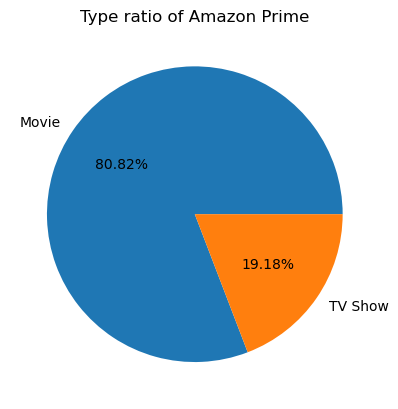
\includegraphics[scale=0.6]{../type_ratio/Amazon Prime_type_ratio.png}
		\end{minipage}
	}
	\subfigure[Disney+]{
		\begin{minipage}[t]{0.45\linewidth}
			\centering
			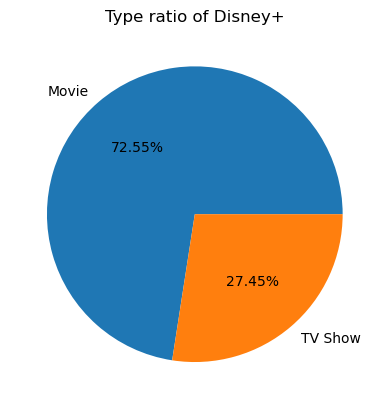
\includegraphics[scale=0.6]{../type_ratio/Disney+_type_ratio.png}
		\end{minipage}
	}
	\subfigure[Hulu]{
		\begin{minipage}[t]{0.45\linewidth}
			\centering
			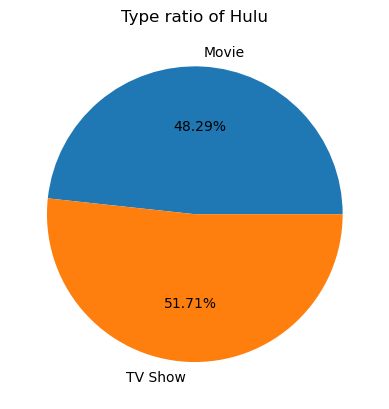
\includegraphics[scale=0.6]{../type_ratio/Hulu_type_ratio.png}
		\end{minipage}
	}
	\subfigure[Netflix]{
		\begin{minipage}[t]{0.45\linewidth}
			\centering
			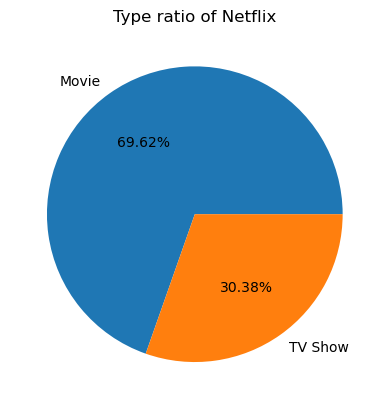
\includegraphics[scale=0.6]{../type_ratio/Netflix_type_ratio.png}
		\end{minipage}
	}
	\caption{The ratio of the material types among the platforms}
	\label{fig:type_ratio}
\end{figure}
	
According to the figure (Fig. \ref{fig:type_ratio}) and the table 
(Tab. \ref{tab:type_ratio}), we can find that Hulu has the most TV shows materials 
ratio, which is 51.71\%. And Hulu is the only one that the TV shows ratio is more 
than 50\%. Amazon Prime has got the least ratio of TV shows, about 19.18\%, which 
is the only one less than 20\%. Therefore, it is quite clear that the content of 
Amazon Prime more rely on movies while that of Hulu more rely on TV shows.

\subsection{Genres of movies and TV shows in every platform}

The column {\it listed\_in} gives information about the movies and TV shows. 
We can find the most genres that the movies and TV shows belong. We get the genres 
data in the following tables (Tab. \ref{tab:amazon_prime_genres}
\ref{tab:disney_plus_genres} \ref{tab:hulu_genres} \ref{tab:netflix_genres}). And 
from these tables, we draw the following figures (Fig. \ref{fig:genres}).
\begin{table}[!htb]
	\centering
	\caption{Popular genres on Amazon Prime}
	\label{tab:amazon_prime_genres}
	\begin{tabular}{@{}ll@{}}
	\toprule
	Genres           & Ratio   \\ \midrule
	Drama            & 20.14\% \\
	Comedy           & 11.46\% \\
	Action           & 9.05\%  \\
	Suspense         & 8.20\%  \\
	Kids             & 5.93\%  \\
	Documentary      & 5.42\%  \\
	Special Interest & 5.35\%  \\
	Other            & 34.45\% \\ \bottomrule
	\end{tabular}
\end{table}

In the figure (Fig. \ref{fig:genres}), each of the four pie charts has a category 
called 'Other', which denotes the many small categories which occupy less than 4\% 
of the whole tags of one platform.

\begin{table}[!htb]
	\centering
	\caption{Popular genres on Disney+}
	\label{tab:disney_plus_genres}
	\begin{tabular}{@{}ll@{}}
	\toprule
	Genres            & Ratio   \\ \midrule
	Family            & 16.16\% \\
	Animation         & 13.86\% \\
	Comedy            & 13.45\% \\
	Action-Adventure  & 11.56\% \\
	Animals \& Nature & 5.32\%  \\
	Coming of Age     & 5.24\%  \\
	Fantasy           & 4.91\%  \\
	Documentary       & 4.45\%  \\
	Other             & 25.04\% \\ \bottomrule
	\end{tabular}
\end{table}
\begin{table}[!htb]
	\centering
	\caption{Popular genres on Hulu}
	\label{tab:hulu_genres}
	\begin{tabular}{@{}ll@{}}
	\toprule
	Genres        & Ratio   \\ \midrule
	Drama         & 13.42\% \\
	Comedy        & 9.81\%  \\
	Adventure     & 8.22\%  \\
	Action        & 8.21\%  \\
	Documentaries & 7.75\%  \\
	Anime         & 4.87\%  \\
	Other         & 47.67\% \\ \bottomrule
	\end{tabular}
\end{table}
\begin{table}[!htb]
	\centering
	\caption{Popular genres on Netflix}
	\label{tab:netflix_genres}
	\begin{tabular}{@{}ll@{}}
	\toprule
	Genres                 & Ratio   \\ \midrule
	International movies   & 14.24\% \\
	Dramas                 & 12.56\% \\
	Comedies               & 8.66\%  \\
	International TV shows & 6.99\%  \\
	Other                  & 57.54\% \\ \bottomrule
	\end{tabular}
\end{table}

\begin{figure}[!htb]
	\centering
	\subfigure[Amazon Prime]{
		\begin{minipage}[t]{0.45\linewidth}
			\centering
			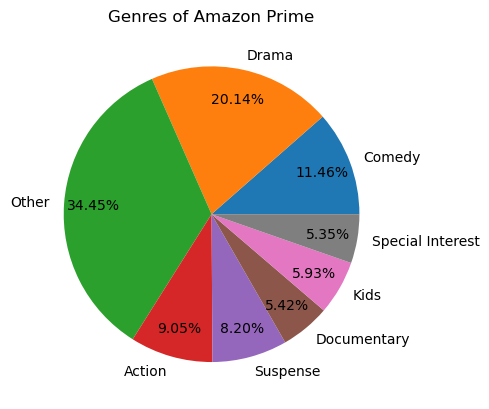
\includegraphics[scale=0.5]{../genres/Amazon Prime_genres.png}
		\end{minipage}
	}
	\subfigure[Disney+]{
		\begin{minipage}[t]{0.45\linewidth}
			\centering
			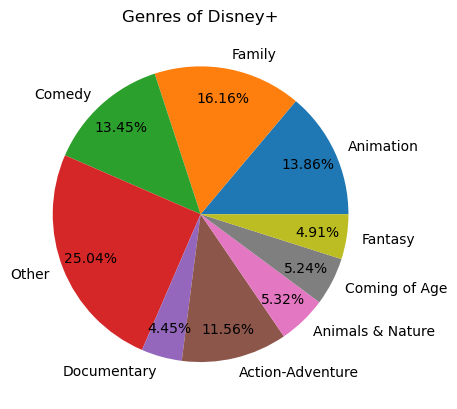
\includegraphics[scale=0.5]{../genres/Disney+_genres.png}
		\end{minipage}
	}
	\subfigure[Hulu]{
		\begin{minipage}[t]{0.45\linewidth}
			\centering
			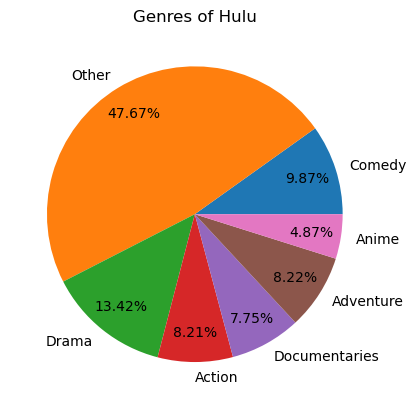
\includegraphics[scale=0.5]{../genres/Hulu_genres.png}
		\end{minipage}
	}
	\subfigure[Netflix]{
		\begin{minipage}[t]{0.45\linewidth}
			\centering
			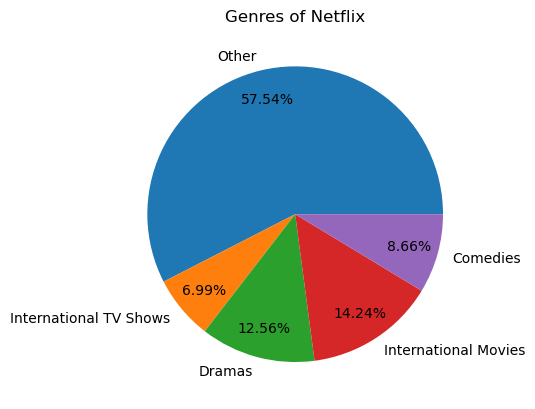
\includegraphics[scale=0.5]{../genres/Netflix_genres.png}
		\end{minipage}
	}
	\caption{The ratio of the material types among the platforms}
	\label{fig:genres}
\end{figure}

As a platform whose target clients are mainly children and 
families, Disney+ is the only one that the first category is not 'Drama' 
(even 'Drama' occupies less than 4\%). And it also has a smallest 'Other', 
about 25\%, which means the platform has a high concentration on other types 
shown in the pie chart.

Among the other platforms except Disney+, the most popular types are 'Drama', 
which has 20.14\% in Amazon Prime, 13.42\% in Hulu, and 12.56\% in Netflix. 
'Comedy' also appears in four pie charts.

\subsection{Release dates of the movies and TV shows}

Since the data has the information about the dates added and the year released, 
we can find the density of the contents added dates for each platform. For 
visualizing this information, some fancy graphs (Fig. 
\ref{fig:added_dates_amazon_prime}
\ref{fig:added_dates_disney_plus}
\ref{fig:added_dates_hulu}
\ref{fig:added_dates_netflix}) 
can be used.

The figure (Fig. \ref{fig:added_dates_amazon_prime}) for Amazon Prime, 
however, lacks of large information so that we only get the results in 2021. As 
for Disney+ (Fig. \ref{fig:added_dates_disney_plus}), we can see that a lot of 
contents were added in November, 2019. In fact, Disney+ was opened at November, 
2019. Therefore, it is not surprised that Disney would put large number of movies 
and TV shows it already had at the very beginning. When it turns to Hulu 
(Fig. \ref{fig:added_dates_hulu}), what we cam observe is Hulu had a quick 
development in recent two years, especially in 2021. Nearly over a half of all 
the movies and TV shows were added in 2021. The last but not least, Netflix 
(Fig. \ref{fig:added_dates_netflix}), has always added many movies and TV shows 
in anytime compared with the other three platforms.

\begin{figure}[!htb]
	\centering
	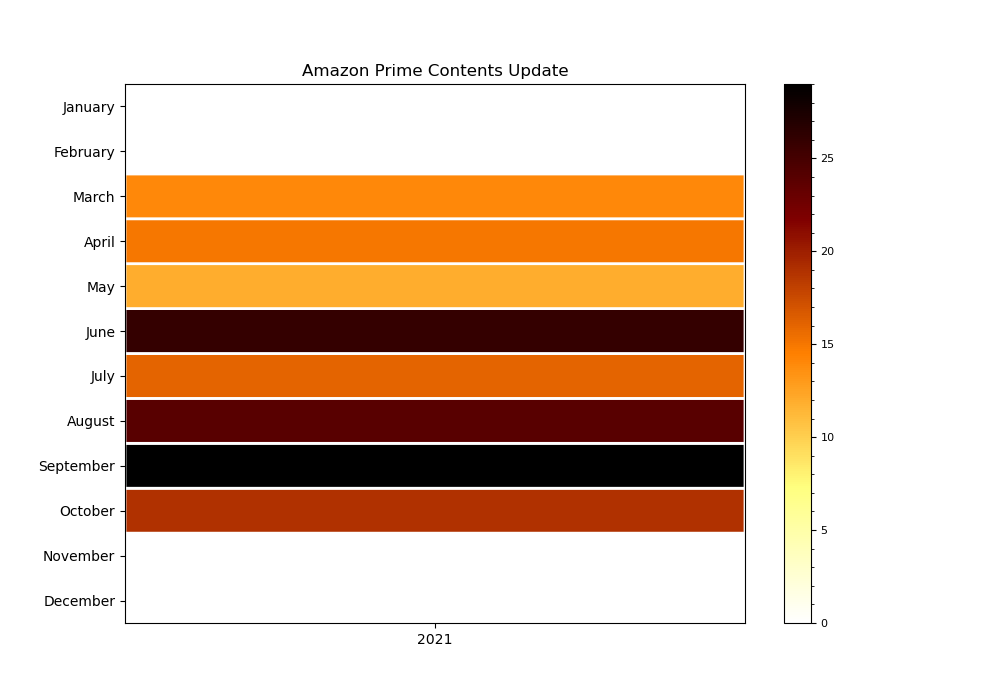
\includegraphics[scale=0.3]{../contents_update/Amazon Prime_contents_update.png}
	\caption{Added dates of Amazon Prime}
	\label{fig:added_dates_amazon_prime}
\end{figure}
\begin{figure}[!htb]
	\centering
	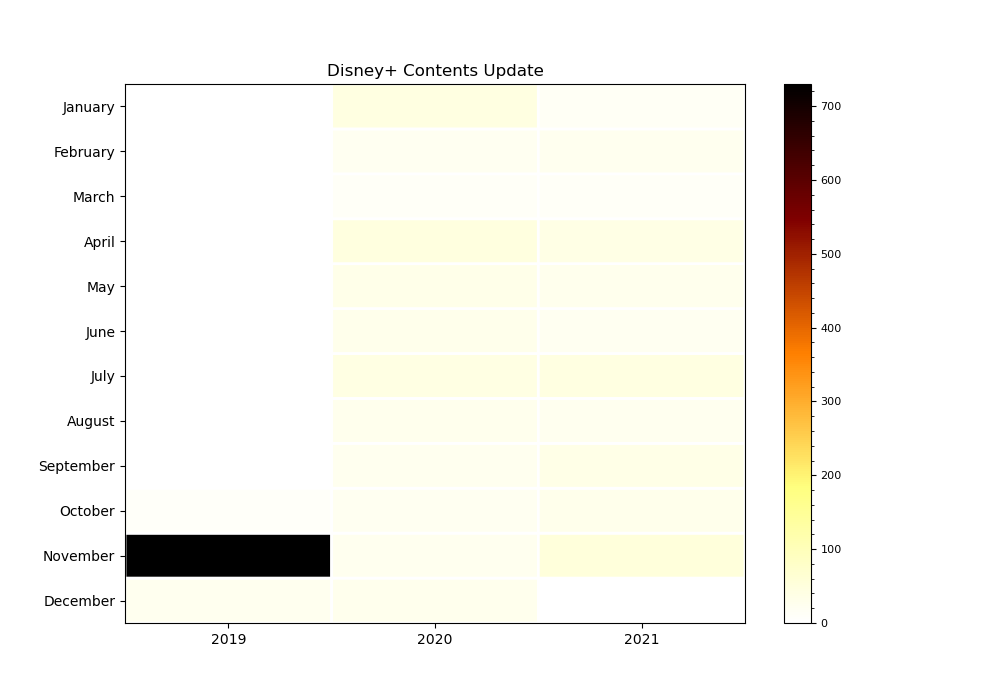
\includegraphics[scale=0.3]{../contents_update/Disney+_contents_update.png}
	\caption{Added dates of Disney+}
	\label{fig:added_dates_disney_plus}
\end{figure}
\begin{figure}[!htb]
	\centering
	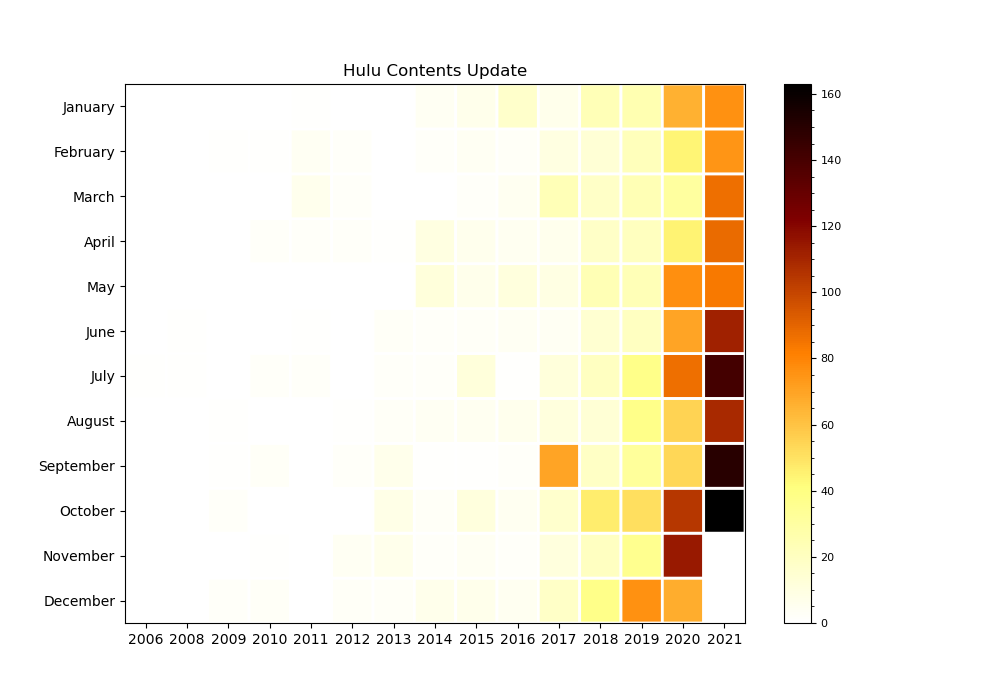
\includegraphics[scale=0.3]{../contents_update/Hulu_contents_update.png}
	\caption{Added dates of Hulu}
	\label{fig:added_dates_hulu}
\end{figure}
\begin{figure}[!htb]
	\centering
	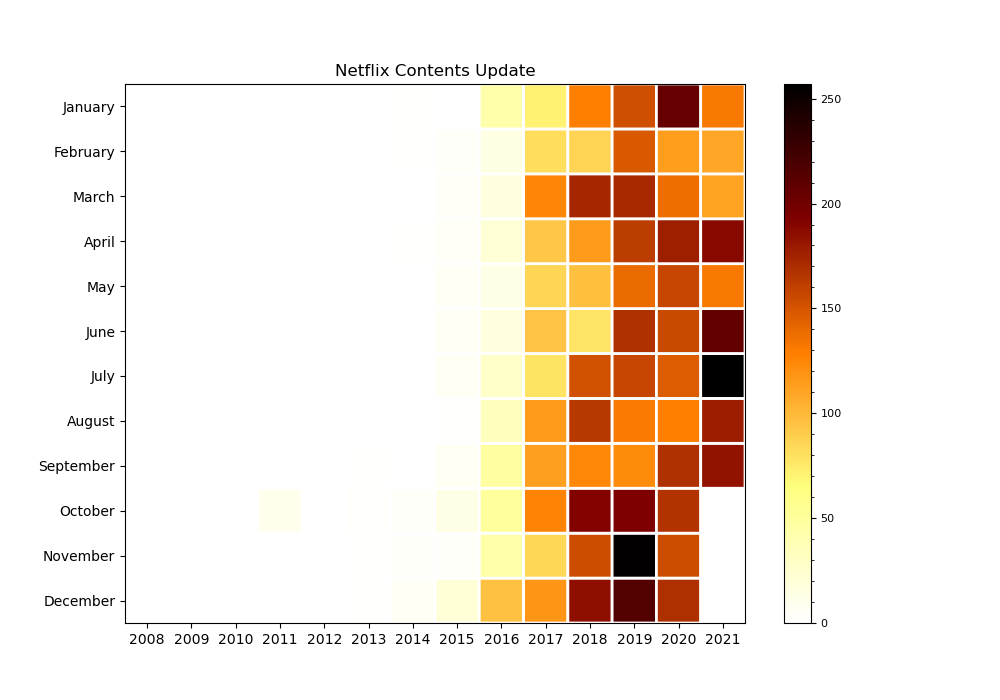
\includegraphics[scale=0.3]{../contents_update/Netflix_contents_update.png}
	\caption{Added dates of Netflix}
	\label{fig:added_dates_netflix}
\end{figure}

\subsection{The distribution of the duration of the movies on all the four platforms}
\label{parag:movie_duration_distribution}

The author of the paper is a fan of movies, who likes enjoying good movies only 
with himself in the films or at home. We can find the duration of all the movies 
and find out the common length of movie time by visualizing the results.

In the figure (Fig. \ref{fig:movie_duration}), we are able to see that the most 
common duration is about between 90 to 120 minutes, where the density is above 1\%.

\begin{figure}[!htb]
	\centering
	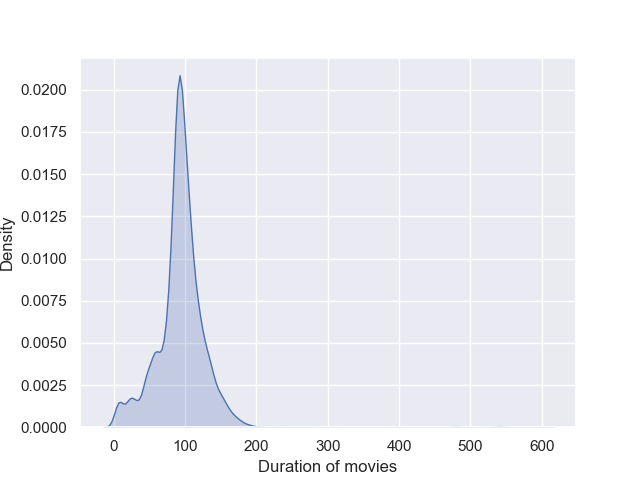
\includegraphics[scale=0.6]{../movie_duration_distribution.png}
	\caption{The distribution of the duration of the online movies}
	\label{fig:movie_duration}
\end{figure}

However, what's surprised is that there exists one movie of which duration is 
more than 600 minutes! The movie is not a regular movie - it is a movie intended 
to help those who have sleep issues. Here is the movie:

\begin{center}
	{\it Soothing Surf at Del Norte for Sleep black screen}
\end{center}

The description of movie is that {\it Black screen reduces the blue-spectrum light 
waves-known to inhibit REM sleep. Awaken rested and refreshed. Accompanied by the 
relaxing ocean surf and natural sounds filmed on location in the remote 
Centerville Beach near the California Redwoods. Great for children, pets and 
anyone with sleep issues. For best results adjust your monitor or TV to the night 
or darkest screen setting.} So, it is not weird to find it a 600-minute movie.

\subsection{The median duration of movies by year}

In the section \ref{parag:movie_duration_distribution}, we find the movie duration
of all the movies. Let's imagine whether there is a connection between the age and 
the movie duration. Will it be longer with the development of movie techniques? 
Or, will it be shorter to fit the metropolitan busy life. At first, the author 
wanted to take the average of the durations of the movies by year. But the author 
realized there might be some extreme values like {\it 601 minutes} in some years. 
By avoiding the impact of extreme values, the author decided to use the median as 
the statistic indicating the durations by year.

\begin{figure}[!htb]
	\centering
	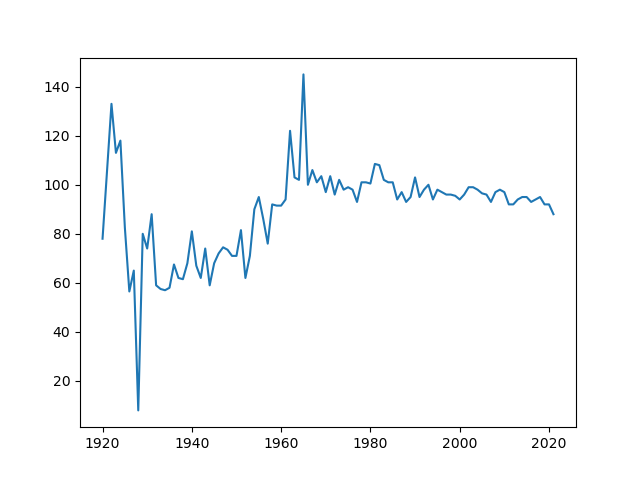
\includegraphics[scale=0.6]{../annual_movie_length_median.png}
	\caption{The median duration of movies by year}
	\label{fig:median_duration_by_year}
\end{figure}

In the figure (Fig. \ref{fig:median_duration_by_year}) we can see that after the 
1970s, when the movie industry became stable, all the medians of durations just 
jump slight around 100 minutes. That is to say, the conclusion we derive in 
\ref{parag:movie_duration_distribution} is quite accurate. 

\section{Producing countries}

In this part, we are going to find the most productive countries in movies and TV 
shows industries. In the table (Tab. \ref{tab:diversity_production}) we can see 
that the most diverse platform among the four platforms is Netflix. There are 
altogether 127 countries involved in the production. The diversity of other three 
platforms is far less than that of Netflix.

\begin{table}[!htb]
	\centering
	\caption{The number of countries involved in the production of four platforms}
	\label{tab:diversity_production}
	\begin{tabular}{@{}ll@{}}
	\toprule
	Platform     & Number of involved countries \\ \midrule
	Amazon Prime & 45                           \\
	Disney+      & 47                           \\
	Hulu         & 57                           \\
	Netflix      & 127                          \\ \bottomrule
	\end{tabular}
\end{table}

Now we are going the most productive five countries of each platform. From (Fig.
\ref{fig:top_produtive_countries_amazon_prime}
\ref{fig:top_produtive_countries_disney_plus}
\ref{fig:top_produtive_countries_hulu}
\ref{fig:top_produtive_countries_netflix}) 
we can see that the United States is absolutely the most productive countries on 
any platform. Besides the United States, India also appears twice and in the 
second place after the United States. The United Kingdom and Canada also appear in 
four figures, which shows that they also have strong entertainment industry.
\begin{figure}[!htb]
	\centering
	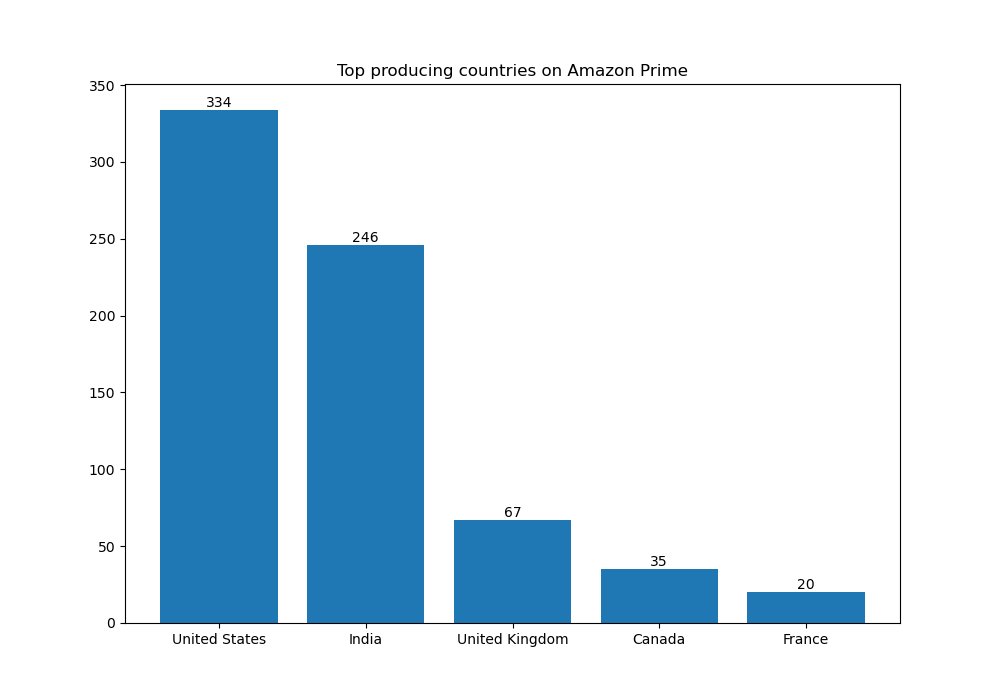
\includegraphics[scale=0.5]{../producing_countries/Amazon Prime_producing_countries.png}
	\caption{Top productive countries on Amazon Prime}
	\label{fig:top_produtive_countries_amazon_prime}
\end{figure}
\begin{figure}[!htb]
	\centering
	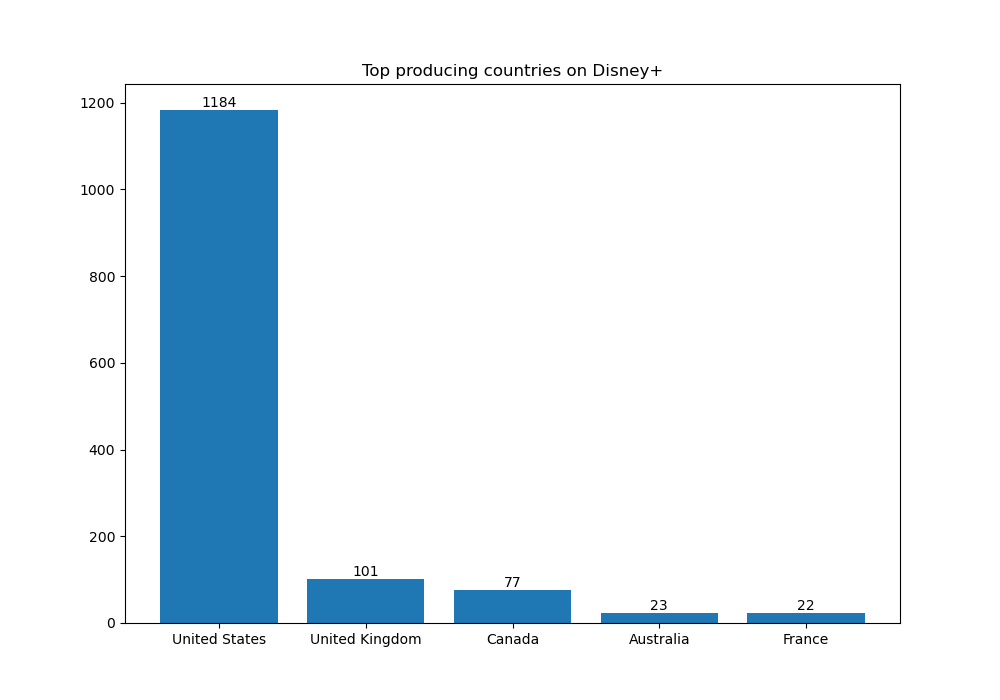
\includegraphics[scale=0.5]{../producing_countries/Disney+_producing_countries.png}
	\caption{Top productive countries on Disney+}
	\label{fig:top_produtive_countries_disney_plus}
\end{figure}
\begin{figure}[!htb]
	\centering
	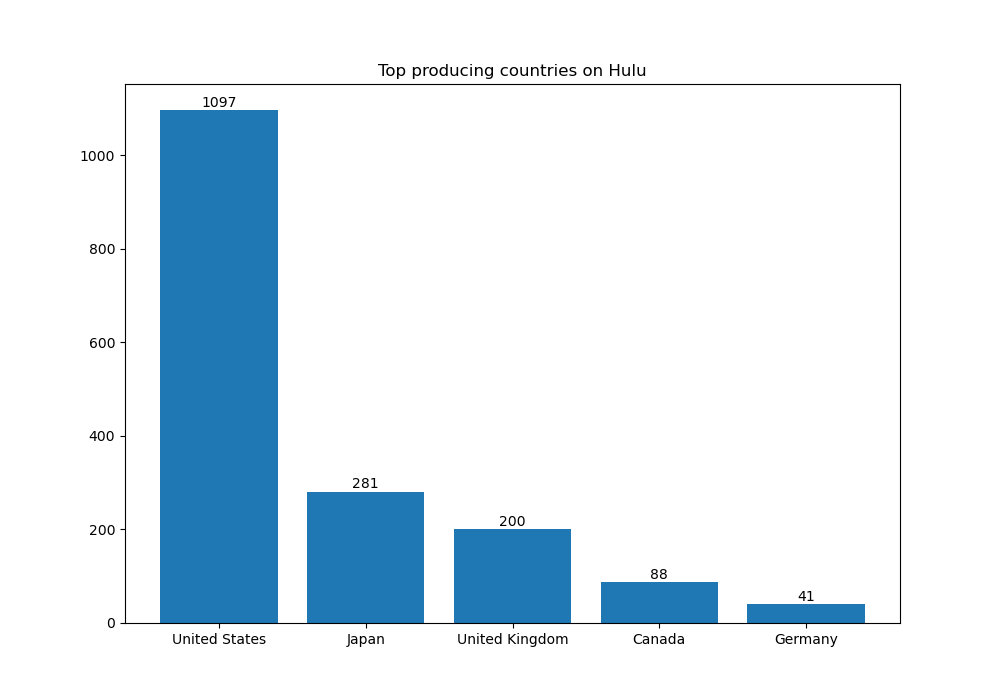
\includegraphics[scale=0.5]{../producing_countries/Hulu_producing_countries.png}
	\caption{Top productive countries on Hulu}
	\label{fig:top_produtive_countries_hulu}
\end{figure}
\begin{figure}[!htb]
	\centering
	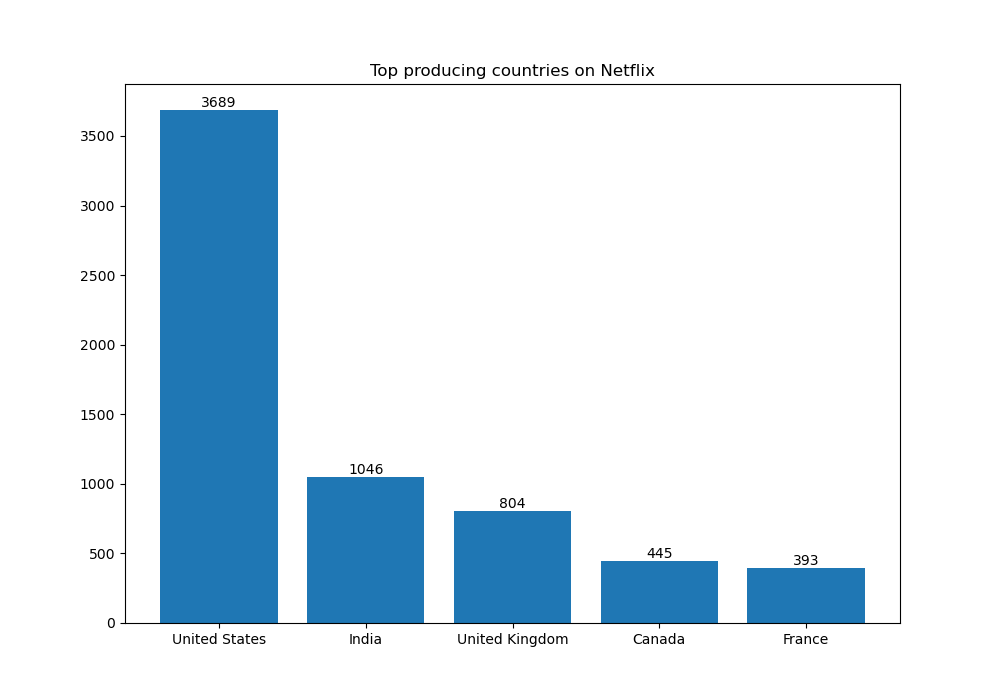
\includegraphics[scale=0.5]{../producing_countries/Netflix_producing_countries.png}
	\caption{Top productive countries on Netflix}
	\label{fig:top_produtive_countries_netflix}
\end{figure}


% \begin{figure}[!htb]
% 	\centering
% 	\subfigure[Amazon Prime]{
% 		\begin{minipage}[t]{0.45\linewidth}
% 			\centering
% 			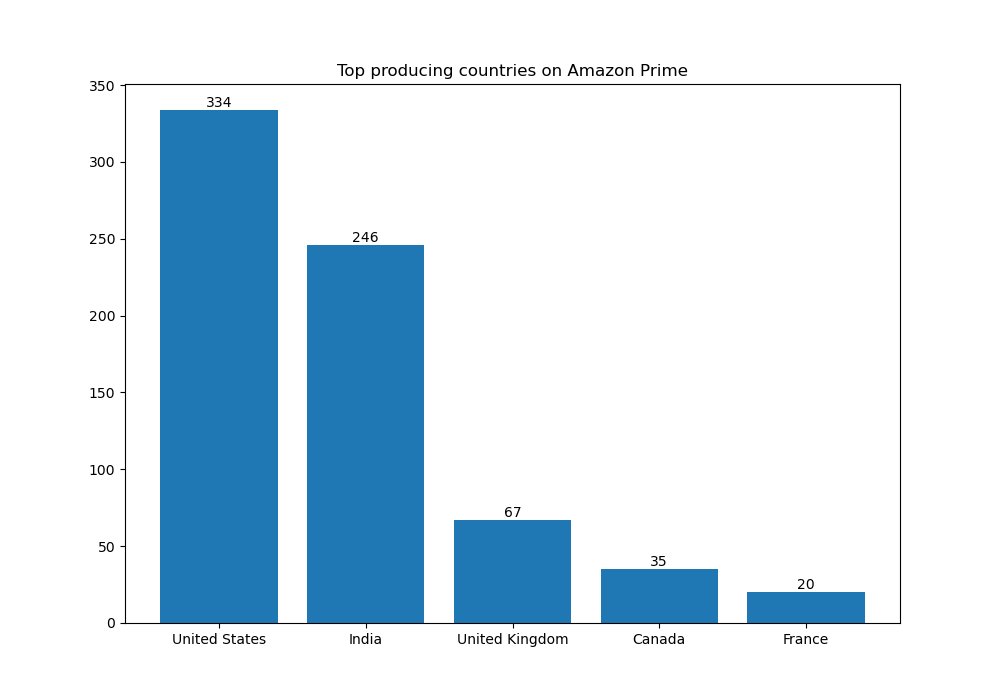
\includegraphics[scale=0.4]{../producing_countries/Amazon Prime_producing_countries.png}
% 		\end{minipage}
% 	}
% 	\subfigure[Disney+]{
% 		\begin{minipage}[t]{0.45\linewidth}
% 			\centering
% 			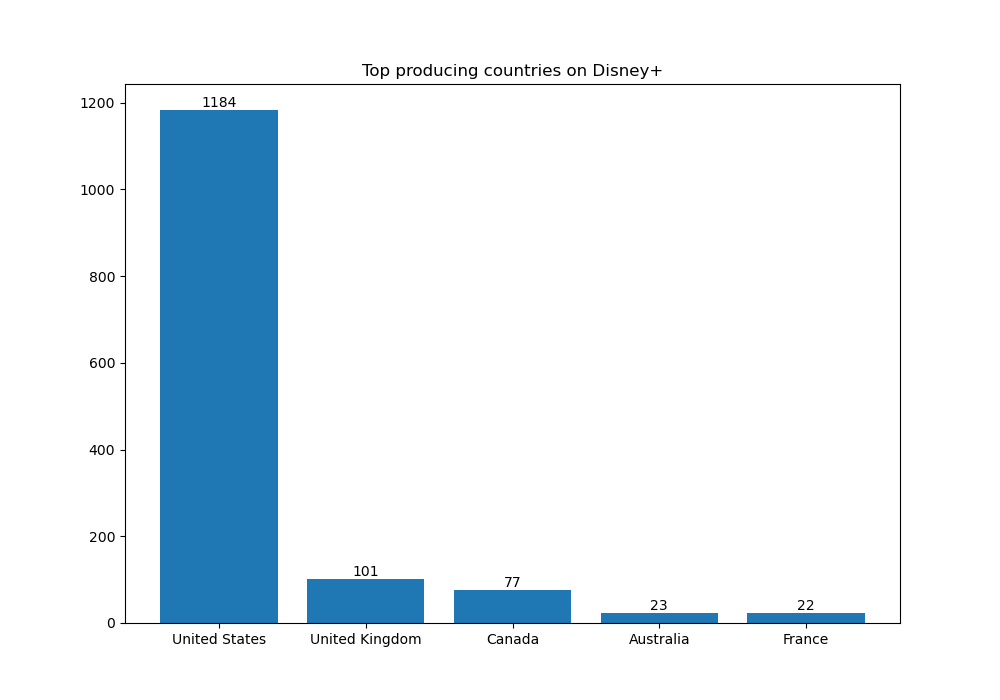
\includegraphics[scale=0.4]{../producing_countries/Disney+_producing_countries.png}
% 		\end{minipage}
% 	}
% 	\subfigure[Hulu]{
% 		\begin{minipage}[t]{0.45\linewidth}
% 			\centering
% 			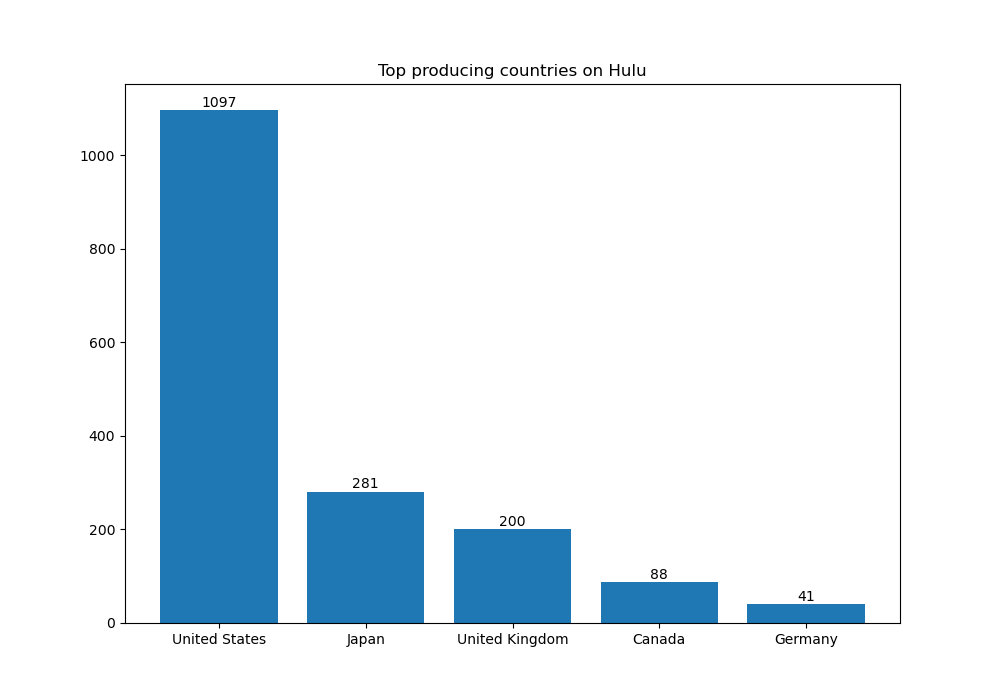
\includegraphics[scale=0.4]{../producing_countries/Hulu_producing_countries.png}
% 		\end{minipage}
% 	}
% 	\subfigure[Netflix]{
% 		\begin{minipage}[t]{0.45\linewidth}
% 			\centering
% 			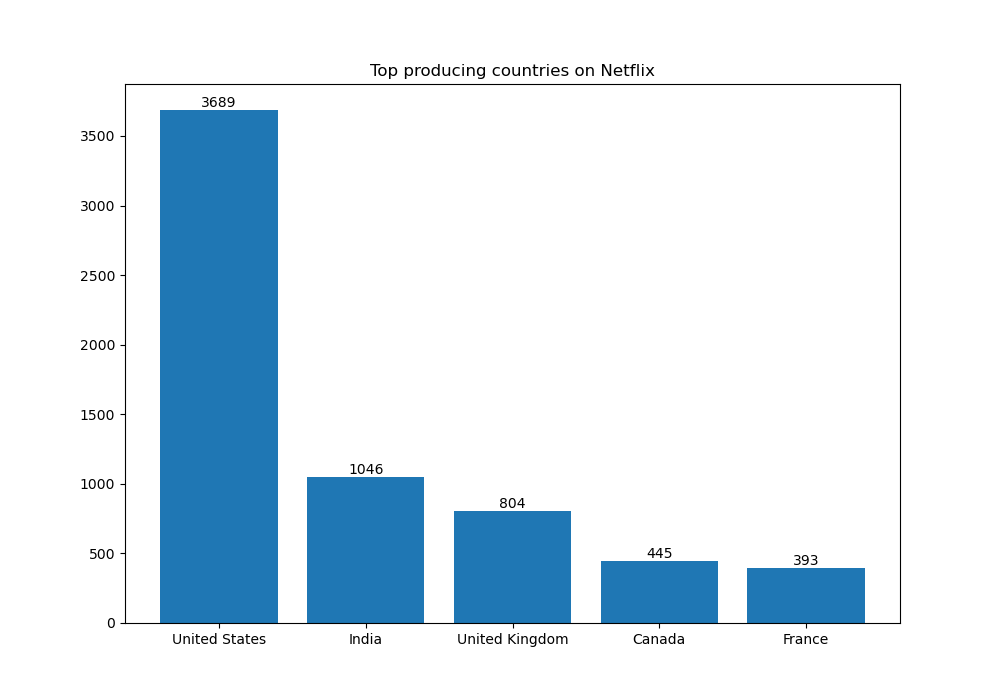
\includegraphics[scale=0.4]{../producing_countries/Netflix_producing_countries.png}
% 		\end{minipage}
% 	}
% 	\caption{The top productive countries of each platform}
% 	\label{fig:top_productive_countries}
% \end{figure}

\section{Operating strategies of each platform}
This is very hard to derive according to these four simple datasets which contain 
only the contents on the platforms. The author decided to focus on the minimum age 
requried to see the contents. In order to quantify the ratings, the author makes a 
mapping standard (Tab. \ref{tab:numerical_ratings}). According to this standard, 
we are able to quantify the suitable ages of all the TV shows and movies of one 
platform and then calculate its average suitable age for one platform.

By using the standard, we can calculate the average minimum age of each platform 
(Fig. \ref{tab:platform_minimum_age}). In the table, we find that only Disney+ 
has clear targets on children, of which the average minimum suitable age is only 
4.72 years old. The other three platforms are quite the same, range from 11.97 to 
13.29 years old.

\begin{table}[!htb]
	\centering
	\caption{The numerical standard of ratings}
	\label{tab:numerical_ratings}
	\begin{tabular}{@{}ll@{}}
	\toprule
	Verbal ratings & Numerical ratings \\ \midrule
	TV-Y           & 2                 \\
	TV-Y7          & 7                 \\
	TV-Y7-FV       & 7                 \\
	TV-G           & 0                 \\
	TV-PG          & 7                 \\
	TV-14          & 14                \\
	TV-MA          & 17                \\
	TV-NR          & numpy.nan         \\
	G              & 0                 \\
	PG             & 7                 \\
	PG-13          & 13                \\
	R              & 17                \\
	NC             & 18                \\
	NR             & numpy.nan         \\
	NOT\_RATE      & numpy.nan         \\
	NOT RATED      & numpy.nan         \\
	UR             & numpy.nan         \\
	UNRATED        & numpy.nan         \\
	ALL            & 0                 \\
	ALL\_AGES      & 0                 \\
	18+            & 18                \\
	AGES\_18\_     & 18                \\
	AGES\_16\_     & 16                \\
	16+            & 16                \\
	16             & 16                \\
	13+            & 13                \\
	7+             & 7                 \\ \bottomrule
	\end{tabular}
\end{table}

\begin{table}[!htb]
	\centering
	\caption{The average minimum age of each platform}
	\label{tab:platform_minimum_age}
	\begin{tabular}{@{}ll@{}}
	\toprule
	Platform     & Minimum age \\ \midrule
	Amazon Prime & 11.97       \\
	Disney+      & 4.72        \\
	Hulu         & 12.25       \\
	Netflix      & 13.29       \\ \bottomrule
	\end{tabular}
\end{table}

Taking a further step, we can generate the wordclouds (Fig. \ref{fig:wordclouds}) 
for all the descriptions on each platform. And we can see that except for Disney+, 
the other three clouds have almost the same topics: life, love, new, family, and 
fried etc.
\begin{figure}[!htb]
	\centering
	\subfigure[Amazon Prime]{
		\begin{minipage}[t]{0.45\linewidth}
			\centering
			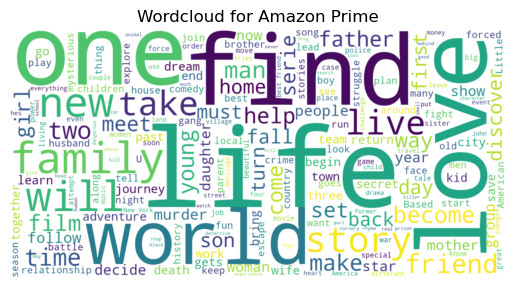
\includegraphics[scale=0.5]{../wordcloud/Amazon Prime_wordcloud.png}
		\end{minipage}
	}
	\subfigure[Disney+]{
		\begin{minipage}[t]{0.45\linewidth}
			\centering
			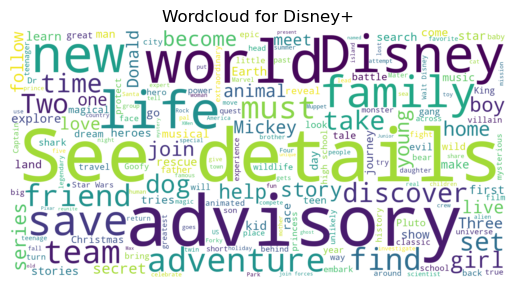
\includegraphics[scale=0.5]{../wordcloud/Disney+_wordcloud.png}
		\end{minipage}
	}
	\subfigure[Hulu]{
		\begin{minipage}[t]{0.45\linewidth}
			\centering
			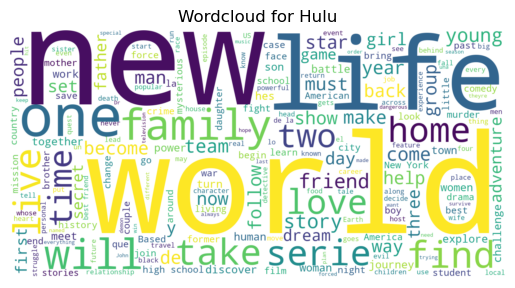
\includegraphics[scale=0.5]{../wordcloud/Hulu_wordcloud.png}
		\end{minipage}
	}
	\subfigure[Netflix]{
		\begin{minipage}[t]{0.45\linewidth}
			\centering
			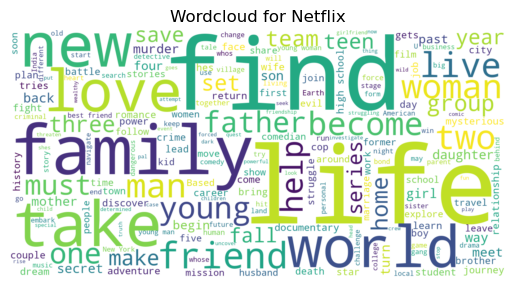
\includegraphics[scale=0.5]{../wordcloud/Netflix_wordcloud.png}
		\end{minipage}
	}
	\caption{The wordclouds of descriptions among the platforms}
	\label{fig:wordclouds}
\end{figure}

\appendix

\section{Appendix}
Here I will post my code. It is hard to control the format.
\newpage
\begin{verbatim}





	
	import pandas as pd
	import numpy as np
	import matplotlib.pyplot as plt
	import seaborn as sns
	import os
	import re
	from wordcloud import WordCloud
	
	pd.options.mode.chained_assignment = None
	
	filenames = ['amazon_prime_titles.csv', 'disney_plus_titles.csv', 'hulu_titles.csv', 'netflix_titles.csv']
	platforms = ['Amazon Prime', 'Disney+', 'Hulu', 'Netflix']
	
	def preprocessing(filenames) -> pd.DataFrame:
		'''
		As is shown in the name... \\
		You have to call this function before all other functions.
		'''
		data = []
		for i in range(len(filenames)):
			data.append(pd.read_csv(filenames[i]))
			data[i].drop(columns=['show_id', 'director', 'cast'], inplace=True)
			'''
				There are dirty data in the column 'rating'.
				Some values in this column denotes the info of 'duration', not 'rating'
				I plan to clean the data here at the very beginning.
			'''
			for index, row in data[i].iterrows():
				if str(row['rating']).endswith('min') or str(row['rating']).endswith('Season') or str(row['rating']).endswith('Seasons'):
					data[i]['duration'][index] = data[i]['rating'][index]
					data[i]['rating'][index] = np.NaN
		return data
	
	# preprocessing is above this line, specific figures and graphs functions are below this line
	
	def type_ratio(data, platforms) -> None:
		'''
		save the ratio of types pie chart of the platforms
		'''
		labels = ['Movie', 'TV Show']
		# plt.axis('off')
		os.system("rm -rf ./type_ratio")
		os.system("mkdir type_ratio")
		for i in range(len(data)):
			num_movie = len(data[i][data[i]['type'] == 'Movie'])
			num_tv_show = len(data[i][data[i]['type'] == 'TV Show'])
			plt.figure()
			plt.pie([num_movie, num_tv_show], labels=labels, autopct='%.2f%%')
			plt.title('Type ratio of {}'.format(platforms[i]))
			plt.savefig('./type_ratio/{}_type_ratio.png'.format(platforms[i]), bbox_inches='tight')
	
	def genres(data, platforms) -> None:
		'''
		save the genres pie chart of the platforms
		'''
		os.system("rm -rf ./genres")
		os.system("mkdir genres")
		for i in range(len(data)):
			topics = {}
			for labels in data[i]['listed_in']:
				for topic in labels.split(', '):
					topics[topic] = topics.setdefault(topic, 0) + 1
	
			# this part is to deal some dirty data
			if 'and Culture' in topics:
				topics['Culture'] = topics['and Culture']
				del topics['and Culture']
	
			thiner_topics = {}
			for k, v in topics.items():
				if v / len(data[i]) >= 0.1:
					thiner_topics[k] = v
				else:
					thiner_topics['Other'] = thiner_topics.setdefault('Other', 0) + v
			# dirty data processing ends
	
			plt.figure()
			plt.title('Genres of {}'.format(platforms[i]))
			plt.pie(thiner_topics.values(), labels=thiner_topics.keys(), autopct='%.2f%%', pctdistance=0.8)
			plt.savefig('./genres/{}_genres.png'.format(platforms[i]), bbox_inches='tight')
	
	def added_date(data, platforms) -> None:
		'''
		save the charts of the adding date of the contents of each platform
		'''
		os.system("rm -rf ./contents_update")
		os.system("mkdir contents_update")
		for i in range(len(data)):
			temp = data[i][['date_added']].dropna()
			temp['year'] = temp['date_added'].apply(lambda x : x.split(', ')[-1])
			temp['month'] = temp['date_added'].apply(lambda x : x.lstrip().split(' ')[0])
			month_order = ['January', 'February', 'March', 'April', 'May', 'June', 'July', 'August', 'September', 'October', 'November', 'December'][::-1]
			df = temp.groupby('year')['month'].value_counts().unstack()
			for month in month_order:
				if month not in set(df.columns):
					df[month] = np.NaN
			df = df.fillna(0)[month_order].T
	
			plt.figure(figsize=(10, 7))
			plt.pcolor(df, cmap='afmhot_r', edgecolors='white', linewidths=2) # heatmap
			plt.xticks(np.arange(0.5, len(df.columns), 1), df.columns)
			plt.yticks(np.arange(0.5, len(df.index), 1), df.index)
	
			plt.title('{} Contents Update'.format(platforms[i]))
			cbar = plt.colorbar()
	
			cbar.ax.tick_params(labelsize=8) 
			cbar.ax.minorticks_on()
			plt.savefig('./contents_update/{}_contents_update.png'.format(platforms[i]))
	
	def minimum_age(data, platforms) -> None:
		'''
		quantify the minimum age to see the contents of each platform
		'''
	
		quantify_ratings = {
			'TV-Y': 2,
			'TV-Y7': 7,
			'TV-Y7-FV': 7,
			'TV-G': 0,
			'TV-PG': 7, # may be unsuitable for younger children
			'TV-14': 14,
			'TV-MA': 17,
			'TV-NR': np.nan,
			'G': 0,
			'PG': 7, # may be not suitale for children
			'PG-13': 13,
			'R': 17,
			'NC-17': 18,
			'NR': np.nan,
			'NOT_RATE': np.nan,
			'NOT RATED': np.nan,
			'UR': np.nan,
			'UNRATED': np.nan,
			'ALL': 0,
			'ALL_AGES': 0,
			'18+': 18,
			'AGES_18_': 18,
			'AGES_16_': 16,
			'16+': 16,
			'16': 16,
			'13+': 13,
			'7+': 7
		}
	
		for i in range(len(data)):
			print('The contents of {} have a mean age at {:.2f}'.format(platforms[i], np.mean(pd.Series([quantify_ratings[rating] for rating in data[i]['rating'].dropna()]).dropna())))
	
	def producing_countries(data, platforms):
		'''
		find the most productive countries
		'''
		os.system("rm -rf ./producing_countries")
		os.system("mkdir producing_countries")
		for i in range(len(data)):
			countries = {}
			for labels in data[i]['country'].dropna():
				# print(labels)
				for country in labels.split(', '):
					countries[country] = countries.setdefault(country, 0) + 1
			countries = sorted(countries.items(), key=lambda kv:(kv[1], kv[0]), reverse=True)
			print('On {}, there are {} countries involved in production.'.format(platforms[i], len(countries)))
			top_countries = []
			top_counts = []
			for name, counts in countries[:5]:
				top_countries.append(name)
				top_counts.append(counts)
			plt.figure(figsize=(10, 7))
			plt.title('Top producing countries on {}'.format(platforms[i]))
			plt.bar(top_countries, top_counts, data=top_counts)
			for country, counts in zip(top_countries, top_counts):
				plt.text(country, counts + 0.05, '%.0f' % counts, ha='center', va='bottom')
			plt.savefig('./producing_countries/{}_producing_countries.png'.format(platforms[i]))
			
	def movie_duration_analysis(data):
		'''
		find the movie durations of all the platforms
		'''
		all_movie_duration = []
		for i in range(len(data)):
			movie_filtered = data[i][data[i]['type'] == 'Movie']
	
			# There are some very dirty data which have 'Seasons' instead of 'min' for movies.
			dirty = movie_filtered[(movie_filtered['duration'].str.endswith('Seasons')) | (movie_filtered['duration'].str.endswith('Season'))].index
			movie_filtered.drop(dirty, inplace=True)
			all_movie_duration.extend(movie_filtered['duration'].dropna().str.replace(' min', '').values.astype(int))
	
		plt.figure()
		sns.set(style='darkgrid')
		sns.kdeplot(data=all_movie_duration, shade=True)
		plt.xlabel('Duration of movies')
		plt.savefig('movie_duration_distribution.png')
	
	def median_movie_duration_by_year(data):
		'''
		find the median of movie durations of all the platforms by year.
		'''
		all_movie_duration = pd.DataFrame(columns=['duration'], index=['release_year'])
		for i in range(len(data)):
			if i == 2:
				continue
			'''
			Here I jump over Hulu due to its dirty table!!!!!
			'''
			movie_filtered = data[i][data[i]['type'] == 'Movie']
			dirty = movie_filtered[(movie_filtered['duration'].str.endswith('Seasons')) | (movie_filtered['duration'].str.endswith('Season'))].index
			movie_filtered.drop(dirty, inplace=True)
			movie_filtered['duration'].dropna(inplace=True)
			movie_filtered['duration'] = movie_filtered['duration'].apply(lambda x: x.replace(' min', ''))
			movie_focus = movie_filtered.drop(columns=['title', 'type', 'country', 'date_added', 'rating', 'listed_in'])
			all_movie_duration = pd.concat([all_movie_duration, movie_focus])
	
		annual_movie_length_median = all_movie_duration.groupby(['release_year']).median()
		plt.plot(annual_movie_length_median.index, annual_movie_length_median['duration'].values)
		plt.savefig('annual_movie_length_median.png')
		
	def description_wordcloud(data, platforms):
		'''
		Make wordclouds of descriptions 
		'''
		os.system("rm -rf ./wordcloud")
		os.system("mkdir wordcloud")
	
		for i in range(len(data)):
			
			descriptions = data[i]['description'].dropna()
			words = []
			for single_movie_description in descriptions:
				single_movie_description.replace(',.?:\'\";', '')
				words += re.sub(r'[^\w\s]', '', single_movie_description).split()
			cloud = WordCloud(width=1600, height=800, background_color='white').generate(' '.join(words))
			plt.axis('off')
			plt.imshow(cloud, interpolation='bilinear')
			plt.title('Wordcloud for {}'.format(platforms[i]))
			plt.savefig('./wordcloud/{}_wordcloud.png'.format(platforms[i]), bbox_inches='tight')
	
	
	data = preprocessing(filenames)
	type_ratio(data, platforms)
	genres(data, platforms)
	added_date(data, platforms)
	minimum_age(data, platforms)
	producing_countries(data, platforms)
	movie_duration_analysis(data)
	median_movie_duration_by_year(data)
	description_wordcloud(data, platforms)
\end{verbatim}
	
\end{document}